\message{ !name(LSDS_project3_hayezl.tex)}\documentclass[a4paper, 11pt]{article}

\usepackage[utf8]{inputenc}
\usepackage[T1]{fontenc}
\usepackage{graphicx, wrapfig}
\usepackage[top=3cm, bottom=3cm, left=3.2cm, right=3.2cm]{geometry}
\usepackage{lmodern}
\usepackage{fancyhdr}
\usepackage{color, colortbl}
\usepackage[usenames, dvipsnames]{xcolor}
\usepackage{amsmath}
\usepackage{amssymb}
\usepackage{mathrsfs}
\usepackage{amsthm}
\usepackage{pgf, pgfplots, tikz}
\usepackage{listings}
\usepackage{makeidx}
\usepackage{hyperref}
\usepackage{setspace}
\usetikzlibrary{calc}
\usetikzlibrary{plotmarks}
\usetikzlibrary{decorations.markings}
\usetikzlibrary{decorations.pathreplacing}
\usepackage{manfnt, multicol}
\usepackage[section]{algorithm}
\usepackage{algorithmicx, algpseudocode, listings}
% fixes a bug for closing parantheses
\usepackage{etoolbox}
\makeatletter
\patchcmd{\lsthk@SelectCharTable}{%
  \lst@ifbreaklines\lst@Def{`)}{\lst@breakProcessOther)}\fi}{}{}{}
\makeatother
\usepackage{array, multirow, longtable}
\usepackage{enumerate}
\usepackage{csquotes}
\usepackage[inline]{enumitem}
\usepackage[english]{babel}
\usepackage{caption, tabu}


%°°°°°°°°°°°°°°°°°°°°°°°°°°°°°°°°°°°°°°°°°°°°°°%
%----Définition de l'environnement listings----%
%°°°°°°°°°°°°°°°°°°°°°°°°°°°°°°°°°°°°°°°°°°°°°°%

\lstset{literate=
  {á}{{\'a}}1 {é}{{\'e}}1 {í}{{\'i}}1 {ó}{{\'o}}1 {ú}{{\'u}}1
  {Á}{{\'A}}1 {É}{{\'E}}1 {Í}{{\'I}}1 {Ó}{{\'O}}1 {Ú}{{\'U}}1
  {à}{{\`a}}1 {è}{{\`e}}1 {ì}{{\`i}}1 {ò}{{\`o}}1 {ù}{{\`u}}1
  {À}{{\`A}}1 {È}{{\'E}}1 {Ì}{{\`I}}1 {Ò}{{\`O}}1 {Ù}{{\`U}}1
  {ä}{{\"a}}1 {ë}{{\"e}}1 {ï}{{\"i}}1 {ö}{{\"o}}1 {ü}{{\"u}}1
  {Ä}{{\"A}}1 {Ë}{{\"E}}1 {Ï}{{\"I}}1 {Ö}{{\"O}}1 {Ü}{{\"U}}1
  {â}{{\^a}}1 {ê}{{\^e}}1 {î}{{\^i}}1 {ô}{{\^o}}1 {û}{{\^u}}1
  {Â}{{\^A}}1 {Ê}{{\^E}}1 {Î}{{\^I}}1 {Ô}{{\^O}}1 {Û}{{\^U}}1
  {œ}{{\oe}}1 {Œ}{{\OE}}1 {æ}{{\ae}}1 {Æ}{{\AE}}1 {ß}{{\ss}}1
  {ç}{{\c c}}1 {Ç}{{\c C}}1 {ø}{{\o}}1 {å}{{\r a}}1 {Å}{{\r A}}1
  {€}{{\EUR}}1 {£}{{\pounds}}1
}

\lstdefinestyle{luaCode}{
  basicstyle=\footnotesize,        	% the size of the fonts that are used for the code
  breakatwhitespace=true,         	% sets if automatic breaks should only happen at whitespace
  breaklines=true,                 	% sets automatic line breaking
  captionpos=t,                    	% sets the caption-position to bottom
  commentstyle=\footnotesize\ttfamily\color{Emerald},    	% comment style
  deletekeywords={...},            	% if you want to delete keywords from the given language
  escapeinside={¦}{¦)},         	% if you want to add LaTeX within your code
  extendedchars=true,              	% lets you use non-ASCII characters; for 8-bits encodings only, does not work with UTF-8
  rulecolor=\color{OliveGreen!80},
  frame=trbl,
  framexleftmargin=10.8pt,
  framexrightmargin=7.2pt,
  keepspaces=true,                 	% keeps spaces in text, useful for keeping indentation of code (possibly needs columns=flexible)
  keywordstyle=\small\bfseries\color{OliveGreen!80},   % keyword style
  language=[5.0]Lua,                 	% the language of the code
  morekeywords={job.position},            	% if you want to add more keywords to the set
  numbers=left,                    	% where to put the line-numbers; possible values are (none, left, right)
  numbersep=3pt,                   	% how far the line-numbers are from the code
  numberstyle=\tiny\color{Gray}, 	% the style that is used for the line-numbers
  resetmargins=false                    % sets margins to 0 in a list
  showspaces=false,                	% show spaces everywhere adding particular underscores; it overrides 'showstringspaces'
  showstringspaces=false,          	% underline spaces within strings only
  showtabs=false,                  	% show tabs within strings adding particular underscores
  stepnumber=2,                    	% the step between two line-numbers. If it's 1, each line will be numbered
  stringstyle=\color{RawSienna},     	% string literal style
  tabsize=2,                       	% sets default tabsize to 2 spaces
  title=\lstname,                   	% show the filename of files included with \lstinputlisting; also try caption instead of title
  xleftmargin=1cm,                      % sets left margin indentation
  xrightmargin=1cm                      % sets right margin indentation
}

\lstdefinestyle{gpCode}{
  basicstyle=\footnotesize,        	% the size of the fonts that are used for the code
  breakatwhitespace=true,         	% sets if automatic breaks should only happen at whitespace
  breaklines=true,                 	% sets automatic line breaking
  captionpos=t,                    	% sets the caption-position to bottom
  commentstyle=\footnotesize\ttfamily\color{Emerald},    	% comment style
  deletekeywords={...},            	% if you want to delete keywords from the given language
  escapeinside={¦}{¦)},         	% if you want to add LaTeX within your code
  extendedchars=true,              	% lets you use non-ASCII characters; for 8-bits encodings only, does not work with UTF-8
  rulecolor=\color{OliveGreen!80},
  frame=trbl,
  framexleftmargin=10.8pt,
  framexrightmargin=7.2pt,
  keepspaces=true,                 	% keeps spaces in text, useful for keeping indentation of code (possibly needs columns=flexible)
  keywordstyle=\small\bfseries\color{OliveGreen!80},   % keyword style
  language=Gnuplot,                 	% the language of the code
  morekeywords={linestyle},            	% if you want to add more keywords to the set
  numbers=left,                    	% where to put the line-numbers; possible values are (none, left, right)
  numbersep=3pt,                   	% how far the line-numbers are from the code
  numberstyle=\tiny\color{Gray}, 	% the style that is used for the line-numbers
  resetmargins=false                    % sets margins to 0 in a list
  showspaces=false,                	% show spaces everywhere adding particular underscores; it overrides 'showstringspaces'
  showstringspaces=false,          	% underline spaces within strings only
  showtabs=false,                  	% show tabs within strings adding particular underscores
  stepnumber=2,                    	% the step between two line-numbers. If it's 1, each line will be numbered
  stringstyle=\color{RawSienna},     	% string literal style
  tabsize=2,                       	% sets default tabsize to 2 spaces
  title=\lstname,                   	% show the filename of files included with \lstinputlisting; also try caption instead of title
  xleftmargin=1cm,                      % sets left margin indentation
  xrightmargin=1cm                      % sets right margin indentation
}


\newcommand{\N}{\mathbb{N}}
\newcommand{\Q}{\mathbb{Q}} 
\newcommand{\R}{\mathbb{R}}
\newcommand{\Z}{\mathbb{Z}} 
\newcommand{\C}{\mathbb{C}}
\renewcommand{\epsilon}{\varepsilon} 
\renewcommand{\phi}{\varphi}


\newcommand{\CodeBrackets}[1]{{\color{RoyalBlue}{#1}}}    % color of parantheses and brackets
\newcommand{\CodeDigits}[1]{{\color{RawSienna}{#1}}} % color of numbers

%change les légendes des listings
\DeclareCaptionFont{white}{\color{white}}
\DeclareCaptionFormat{listing}{%
  \centering
  {\colorbox{OliveGreen!80}{%
      \parbox{0.9\linewidth}{%
          \centering
          #1#2#3
        }
      }
    }
  }
\captionsetup[lstlisting]{%
  format=listing,
  labelfont=white,
  textfont=white, 
  singlelinecheck=false, 
  indention=0pt,
  margin=0pt, 
  font={bf,sf,small}
}


%%%%%%%%	Définitions des environnements de théorèmes	%%%%%%%%
%% style théorème, lemme, proposition
\theoremstyle{plain}


%% style définitions, exemples et remarques
\theoremstyle{definition}


% For syncronisation with skim
\synctex = 1



%\title{{\bfseries Large-Scale Distributed Systems}\\ {\Large Project 1: Gossip-based dissemination, Peer
%    Sampling System}}
\title{%
  \normalfont{\bfseries{\rule{\linewidth}{2pt} Large-Scale Distributed Systems\\Project 3: Firefly-inspired synchronization\\ %
    \vspace{-0.4cm}  \rule{\linewidth}{2pt}}}
  }
\author{Laurent \textsc{Hayez}}
% Remove command to get current date 
\date{\today}


\begin{document}

\message{ !name(LSDS_project3_hayezl.tex) !offset(-3) }




\renewcommand{\proofname}{{\scshape Proof}}
\renewcommand{\labelitemi}{\textbullet}


\maketitle

\renewcommand{\contentsname}{Table of contents}
%Table of contents
\tableofcontents



%%  Section 1: Introduction
\section{Introduction}
\label{sec:introduction}

  In nature, fireflies produce light in order to attract mates or prey. One interesting feature of these
  beetles is that when they emit light in group, at some point, they do it in a synchronized manner, just by
  looking at when their neighbours emit light. This feature is interesting in large-scale distributed systems,
  as synchronization might be required, but one node does not know every other nodes. 

  The objective is thus to inspire ourselves from fireflies to try to synchronize nodes in a decentralized
  manner. At first we will detail the protocol skeleton and explain how the core of the protocols will
  work. Then we will look at a two models called ``phase-advance'' and ``phase-delay'' and briefly analyze
  them. The main and final part will be the ``adaptive Ermentrout model'' which is more representative of
  the reality. We will explain the implementation specifities and analyze this model in different situations.
  
  
%% Section 2: Skeleton

\section{Protocol skeleton}
\label{sec:impl-skel}

  According to the paper ``Firefly-inspired Heartbeat Synchronization in Overlay Networks'', the skeleton for
  the different algorithms is composed of two main functions, namely \textsc{activeThread} and
  \textsc{passiveThread}. We provide the pseudo code for the implementation in Algorithm
  \ref{alg:firefly-skeleton}.

  In the different protocols, a node is an oscillator characterized by its phase $\phi$ and the cycle length
  $\Delta$. We define $\phi$ as a sawtooth function with domain $[0,1]$ such that $\frac{d\phi}{dt} =
  \frac{1}{\Delta}$. This is represented in Figure \ref{fig:repr-phi}.

  When $\phi$ reaches $1$, the node will send a flash to a set of neighbour nodes, and $\phi$ is reset to
  $0$. The cycle length, depending on the model chosen, can be the same or different for all nodes. The
  function \textsc{updatePhi} will differ in our implementations, but we will come back on this when needed.

  The core of the synchronization protocol is the function \textsc{processFlash}, i.e. what a node does when it
  receives a flash. This function is responsible of how $\phi$ is updated. Depending on the implementation,
  $\phi$ will be updated, or $\Delta$ will be updated and will affect $\phi$.

  The underlying overlay network protocol used for a node to know its neighbours is the Peer Sampling Service
  (PSS).
  

  \begin{figure}[h]
    \centering
    \begin{tikzpicture}
      % Axis
      \draw[->, >=latex] (-1, 0) -- (10, 0) node[right]{time};
      \draw[->, >=latex] (0, -1) -- (0, 4);
      % Function phi
      \draw (0,0) -- (2, 2) (2, 0) -- (4, 2) (4, 0) -- (6, 2) (6, 0) -- (8, 2) (8, 0);
      \draw[dashed] (2,2) -- (2,0) (4, 2) -- (4, 0) (6, 2) -- (6, 0) (8,2) -- (8,0);
      \draw (7, 1) node[above left]{$\phi$};
      % draw the fires
      \draw[color = BrickRed, ->, >=latex] (2,2) to node[near end, above, rotate=90]{Fire!} (2, 3);
      \draw[color = BrickRed, ->, >=latex] (4,2) to node[near end, above, rotate=90]{Fire!} (4, 3);
      \draw[color = BrickRed, ->, >=latex] (6,2) to node[near end, above, rotate=90]{Fire!} (6, 3);
      \draw[color = BrickRed, ->, >=latex] (8,2) to node[near end, above, rotate=90]{Fire!} (8, 3);
      % draw delta
      \draw[decorate, decoration = {brace, amplitude=10pt, mirror}, yshift = -4pt] (0,0) -- (2, 0) node [midway,
      yshift = -0.8cm] {$\Delta$};
      % draw tick 1 on y axis
      \draw (-0.1, 2) -- (0.1, 2) node[near start, left]{$1$};
      \draw[dashed, color=gray!60] (0,2) -- (10, 2);
      % draw dphi/dt = 1/delta
      \draw (1.5,1.5) node[above left, rotate=45]{$\frac{d\phi}{dt} = \frac{1}{\Delta}$};
    \end{tikzpicture}
    \caption{Representation of $\phi$ and its relation with $\Delta$}
    \label{fig:repr-phi}
  \end{figure}

  
   \begin{algorithm}
     \caption{Skeleton for the Firefly algorithms}
     \label{alg:firefly-skeleton}
     \begin{algorithmic}
       \State \textbf{Variables:}
       \State $\phi$ \Comment phase
       \State $\Delta$ \Comment cycle length 
       \State update\_phi\_period $= \begin{cases} \frac{\Delta}{10} & \text{if } \Delta < 1 \\
         \frac{1}{10\Delta} & \text{if } \Delta \geq 1 \end{cases}$
       \State
       \Function{sendFlash()}{}
         \State $P \gets$ view from PSS
         \State send flash to all peers in $P$
       \EndFunction
       \State
       \Function{processFlash()}{}
         \State depends on the implementation
       \EndFunction
       \State
       \Function{updatePhi()}{}
         \If{$\phi < 1$}
           \State $\phi \gets \phi + \frac{1}{\Delta} \cdot $update\_phi\_period
         \Else
           \State fire event ``Flash!''
           \State $\phi \gets 0$
           \State start new thread \textsc{activeThread}
         \EndIf
       \EndFunction
       \State
       \Function{activeThread()}{}
          \State wait for the event ``Flash!''
          \State sendFlash()
       \EndFunction
       \State
       \Function{passiveThread()}{}
         \State receive flash
         \State processFlash()
       \EndFunction
     \end{algorithmic}
   \end{algorithm}


   We briefly discuss how the protocol skeleton works before we move to the implementation of the
   phase-advance and phase-delay protocols.

   For every implementations, we start by initializing the PSS at each node, and wait two minutes to have a
   consistent view. Then we start a thread \textsc{activeThread} and a periodic thread \textsc{updatePhi}. As
   we defined $\phi$ to be such that $\frac{d\phi}{dt} = \frac{1}{\Delta}$, we have $\phi = \int \phi dt$,
   which explains how we update $\phi$. If $\phi \geq 1$, we fire the event ``Flash!'' that triggers
   \textsc{activeThread} to send that it emitted a flash to the nodes in its view. In \textsc{updatePhi}, we
   then set $\phi$ to 0, as in Figure \ref{fig:repr-phi} and call \textsc{activeThread} to wait for a new
   flash.

   

\section{Phase-advance and phase-delay protocols}
\label{sec:phase-ad-phase-de}

  \subsection{Implementation}
  \label{sec:implementation}

    The fundamental difference with the protocol skeleton here is the implementation of the
    \textsc{processFlash} function. As the two protocols are almost the same, we added the boolean
    \textsc{phase\_advance} to signify the usage of the phase-advance or phase-delay protocol. The pseudo-code
    of the implementation is given in Algorithm \ref{alg:firefly-phase}.

    \begin{algorithm}
     \caption{processFlash for the phase-advance and phase-delay protocols}
     \label{alg:firefly-phase}
     \begin{algorithmic}
       \State \textbf{Variables:}
       \State phase\_advance $\gets$ true or false      
       \State
       \Function{processFlash()}{}
         \If{phase\_advance}
           \State $\phi \gets 1$
         \Else
           \State $\phi \gets 0$
         \EndIf
       \EndFunction
     \end{algorithmic}
   \end{algorithm}



   \subsection{Analysis of the protocols}
   \label{sec:analysis-protocols}

     We tried our implementation with 100 nodes per experiment and $\Delta = 1, 2$ and $5$. For the
     PSS, we used a view of $10$ peers with a period of $20$ seconds for each update. We used a random
     selection for the peer selection, and we used a swapping parameter of $3$ and a healing parameter of $2$
     for the view exchange policy. 

     We start by analyzing the convergence of the phase-advance protocol. On Figure \ref{fig:pa-sync-d1}, we
     can see that from time to time, the protocol seems to synchronize, it does not converge to a stable state
     where all the nodes emit flashes at the same time. In fact, what happens is what we see on Figures
     \ref{fig:pa-sync-d2} and \ref{fig:pa-sync-d5}. Whenever a node flashes, it tells ten other nodes, that set
     $\phi$ to $1$, emit a flash, tell ten other nodes, which emit a flash and so on. We thus have an
     exponential growth of the flash rate which makes the memory used explode very fast. In the logs, we had
     this very error:

     \begin{displayquote}
       \texttt{17:37:43.276437 (66)  Too much memory used: wants 2097182 (max: 2097152), end of process.}
     \end{displayquote}

     This model is therefore highly impratical because it overloads the network very quickly. By analogy with
     fireflies, at first a few fireflies would emit light, and then by observing the neighbours they would
     emit light every time they see a neighbour emitting light, quickly resulting in emitting light constantly, which
     does not happen in reality. 

     \begin{figure}[h]
       \centering
       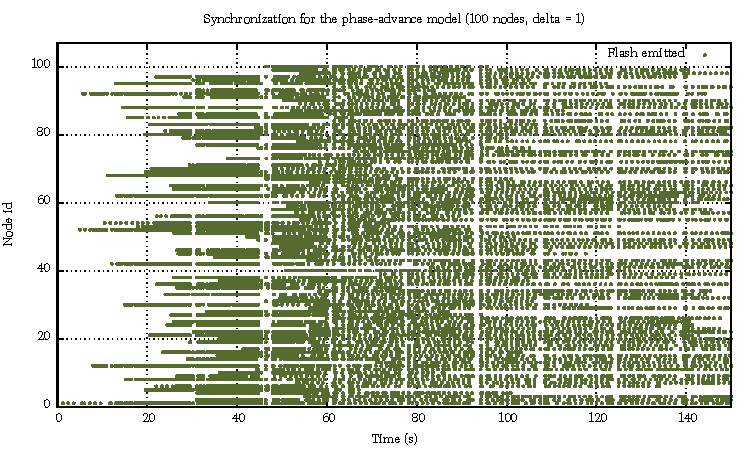
\includegraphics[scale=0.8]{../Plots/Firefly-pa-100nodes-1-9.pdf}
       \caption{Phase-advance model synchronization with $\Delta = 1$}
       \label{fig:pa-sync-d1}
     \end{figure}

     \begin{figure}[h]
       \centering
       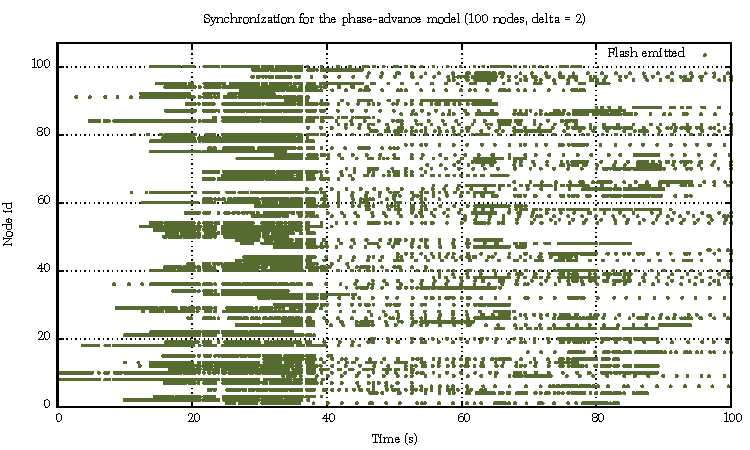
\includegraphics[scale=0.8]{../Plots/Firefly-pa-100nodes-2-6.pdf}
       \caption{Phase-advance model synchronization with $\Delta = 2$}
       \label{fig:pa-sync-d2}
     \end{figure}

      \begin{figure}[h]
       \centering
       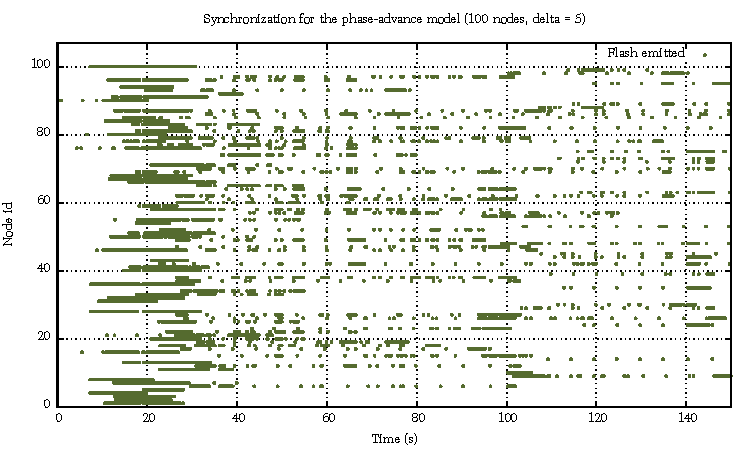
\includegraphics[scale=0.8]{../Plots/Firefly-pa-100nodes-5-3.pdf}
       \caption{Phase-advance model synchronization with $\Delta = 5$}
       \label{fig:pa-sync-d5}
     \end{figure}


     Now let's take a look at the phase-delay model. On Figures \ref{fig:pd-sync-d1} and \ref{fig:pd-sync-d2},
     we representend the emissions for $\Delta = 1$ and $\Delta = 2$ respectively. On both figures we cannot
     distinguish a convergence in the flash emissions. On Figure \ref{fig:pd-sync-d5} however, we can see that
     from 150 seconds after the first flash, the nodes that emit flashes are synchronized. 

     \begin{figure}[h]
       \centering
       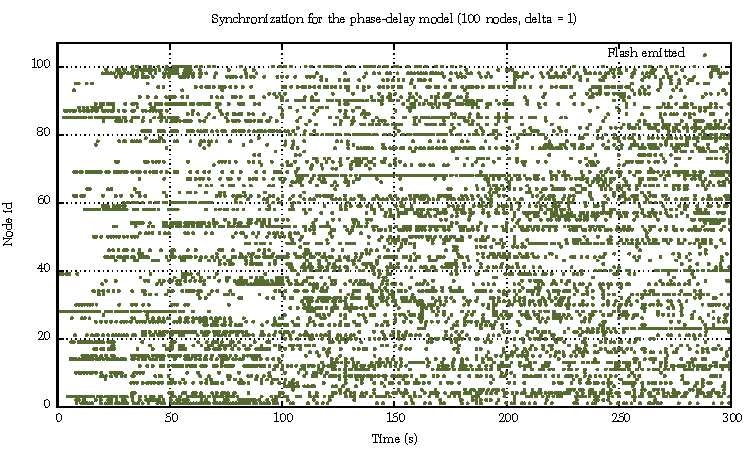
\includegraphics[scale=0.8]{../Plots/Firefly-pd-100nodes-1-6.pdf}
       \caption{Phase-delay model synchronization with $\Delta = 1$}
       \label{fig:pd-sync-d1}
     \end{figure}

     \begin{figure}[h]
       \centering
       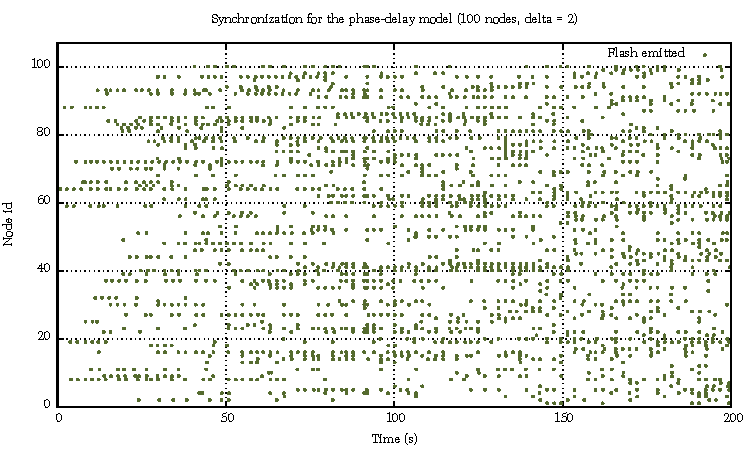
\includegraphics[scale=0.8]{../Plots/Firefly-pd-100nodes-2-4.pdf}
       \caption{Phase-delay model synchronization with $\Delta = 2$}
       \label{fig:pd-sync-d2}
     \end{figure}

      \begin{figure}[h]
       \centering
       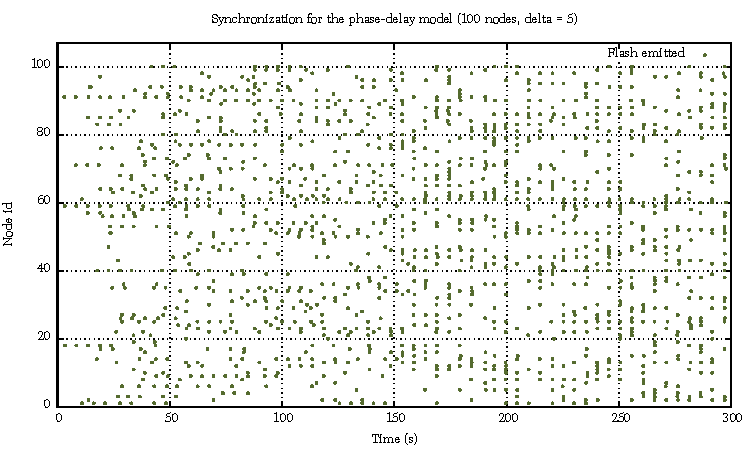
\includegraphics[scale=0.8]{../Plots/Firefly-pd-100nodes-5-5.pdf}
       \caption{Phase-delay model synchronization with $\Delta = 5$}
       \label{fig:pd-sync-d5}
     \end{figure}
     
     Although we seem to obtain some synchronization for $\Delta = 5$, the phase-delay protocol is not
     guaranteed to converge to a stable state where all the nodes are synchronized. Both phase-advance and
     phase-delay protocols rely on the assumption that when a message is sent, it is instantly received. In
     practice, this assumption is highly unrealistic due to packet loss, congestion or simply because even the
     fastest networks, a message is not instantly delivered.

     In our experiments, we considered $\Delta$ to be fixed and the same at all nodes. This assumption does
     not represent reality either; why would all fireflies emit light at the same rate? If we had different
     $\Delta$s at all nodes, or if the skew of the clocks is important, none of the models is guaranteed to
     converge, and it is rather logical as we don't update $\Delta$. If a node starts with $\Delta = 4.5$ and
     another with $\Delta = 5.5$, they will never synchronize. Therefore, both phase-advance and phase-delay
     are mathematically insufficient to model the reality.



\section{Adaptive Ermentrout model}
\label{sec:adapt-ermentr-model}

  According to our preceding conclusion, we now consider a model that allows the node to initally have
  different cycle lengths. This model is called the ``adaptive Ermentrout model''. In this model, we denote by
  $i$ the $i$-th node in the system. Each node has an initial cycle length $\delta_i$ and a natural cycle
  length $\Delta$ which are bounded below and above, ie $\delta_i, \Delta \in (\Delta_l, \Delta_u)$. If there
  is no interaction with other nodes, a node will flash every $\Delta$ seconds. 

  Furthermore, we do not express the model in terms of the cycle length, but rather in terms of the frequency
  $\omega_i = \frac{1}{\delta_i}$. We have $\Omega = \frac{1}{\Delta}$, $\Omega_l = \frac{1}{\Delta_u}$ and
  $\Omega_u = \frac{1}{\Delta_l}$.

  \subsection{Implementation}
  \label{sec:implementation-1}

    The main difference with the phase-advance and phase-delay models is that the function
    \textsc{processFlash} does not update $\phi$, but the frequency $\omega_i$. If a flash arrives when $\phi
    < \frac{1}{2}$ (too late), the frequency will be decreased, and if a flash arrives when $\phi >
    \frac{1}{2}$ (too early), the frequency will be augmented, meaning that a node will ajust its frequency
    according to the flashes it receives. In addition to that, we add a new parameter $\epsilon$ which
    we set to $0.01$ and which represent the offset of the frequency when we update it. The pseudo-code of the
    algorithm is given in Algorithm \ref{alg:adapt-er} (note that the pseudo-code given is what to add/modify
    from the skeleton protocol).


    \begin{algorithm}
     \caption{Pseudo-code for the adaptive Ermentrout model}
     \label{alg:adapt-er}
     \begin{algorithmic}
       \State \textbf{Variables:}
       \State $\Delta_l,\ \Delta,\ \delta_i,\ \Delta_u\ \gets\ 4.5,\ 5,\ \mathrm{rand}(\Delta_l, \Delta_u),\
       5.5$ 
       \State $\Omega_l,\ \Omega,\ \omega_i, \Omega_u\ \gets\ \frac{1}{\Delta_u},\ \frac{1}{\Delta},\
       \frac{1}{\delta_i},\ \frac{1}{\Delta_l}$
       \State $\epsilon \gets 0.01$
       \State
       \Function{processFlash()}{}
         \State $\omega_i \gets \omega_i + \epsilon(\Omega - \omega) + g^+(\phi)(\Omega_l - \omega) +
         g^-(\phi)(\Omega_u - \omega)$
       \EndFunction
       \State
       \State $g^+(\phi) \gets \max \left( \frac{\sin(2\pi \phi)}{2\pi}, 0 \right)$
       \State $g^-(\phi) \gets -\min \left( \frac{\sin(2\pi \phi)}{2\pi}, 0 \right)$
       \State
       \Function{updatePhi()}{}
         \If{$\phi < 1$}
           \State $\phi \gets \phi + \omega_i \cdot $update\_phi\_period
         \Else
           \State fire event ``Flash!''
           \State $\phi \gets 0$
           \State start new thread \textsc{activeThread}
         \EndIf
       \EndFunction
     \end{algorithmic}
   \end{algorithm}


   The functions $g^+$ and $g^-$ formalize the idea that if a flash arrives ``too late'' (respectively ``too
   early''), we must deacrease the frequency (respectively increase it). Indeed we have that
   \[
   g^+(\phi) = 
   \begin{cases}
     0 < a \leq \frac{1}{2\pi} & \text{if } \phi < \frac{1}{2}\\
     0 & \text{if } \phi \geq \frac{1}{2}
   \end{cases},\quad
   g^-(\phi) = 
   \begin{cases}
     0 < a \leq \frac{1}{2\pi} & \text{if } \phi > \frac{1}{2}\\
     0 & \text{if } \phi \leq \frac{1}{2}
   \end{cases}.
   \]

   
    
   \subsection{Analysis of the protocol}
   \label{sec:analysis-protocol-er}

     The setup for this experiment was a network of $64$ nodes. We used $\Delta_l = 4.5$ sec, $\Delta_u = 5.5$
     sec, $\Delta = 5$ sec and $\delta_i$ a random number between $\Delta_l$ and $\Delta_u$. The settings for
     the peer sampling service are the same as for the previous experiment. To plot the figure in
     this section we used the Python scripts \texttt{Parser-synchronization.py} and
     \texttt{Parser-ultimate.py}, and the bash scripts \texttt{Parse-and-plot-sync.sh} and
     \texttt{Parse-and-} \texttt{plot-ultimate.sh}. The bash scripts call the python scripts and the gnuplot script to
     plot the graphs.
     
     \begin{figure}[h]
       \centering
       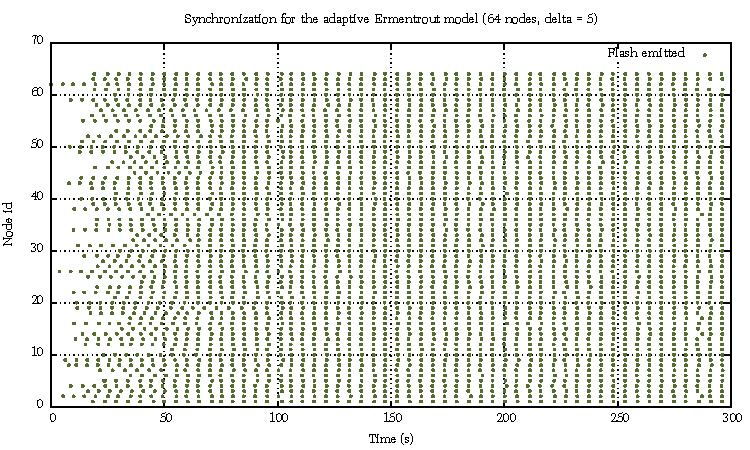
\includegraphics[scale=0.8]{../Plots/Firefly-er-64nodes-d5-2.pdf}
       \caption{Adaptive Ermentrout model synchronization}
       \label{fig:er-sync}
     \end{figure}


     On Figure \ref{fig:er-sync}, we represented how the node synchronize under the adaptive Ermentrout
     model. We clearly see that after 50 seconds, when most of the nodes joined the network, the nodes reaches
     a stable state where the emit light at the same time.

     \begin{figure}[h]
       \centering
       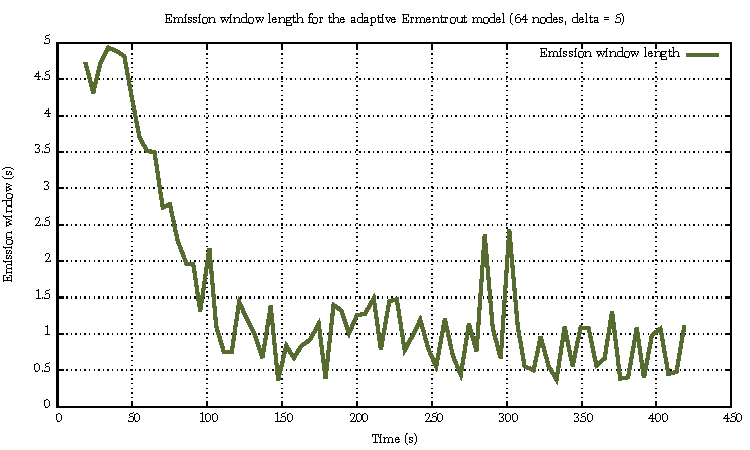
\includegraphics[scale=0.8]{../Plots/Firefly-er-64nodes-d5-2-ewl.pdf}
       \caption{Adaptive Ermentrout model emission window length}
       \label{fig:er-ewl}
     \end{figure}

     On Figure \ref{fig:er-ewl}, we represented the emission window length according to the time. As expected,
     the emission window length reduces as time increases, which indicates that the algorithm converges to a
     stable state. There are some fluctuations however, but the general trend is to decrease and converge to
     somewhere between $0.5$ and $1$ second. On Figure \ref{fig:er-cl}, we plotted the cycle length for each
     node according to the time. The fluctuations can be explained with the cycle length, because we see that
     when there are fluctuations for the emission window length, we have some weird values for the cycle
     lengths, explaining the occasional desynchronization. This could be because the nodes on the cluster were
     overloaded at this time.

     \begin{figure}[h]
       \centering
       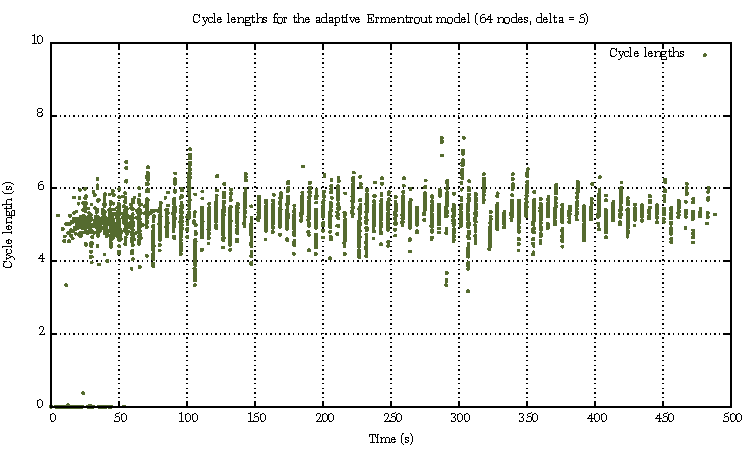
\includegraphics[scale=0.8]{../Plots/Firefly-er-64nodes-d5-2-cl.pdf}
       \caption{Adaptive Ermentrout model cycle length}
       \label{fig:er-cl}
     \end{figure}


   \subsection{Analysis of the protocol under churn}
   \label{sec:analys-prot-under-churn}

     

     \begin{figure}[h]
       \centering
       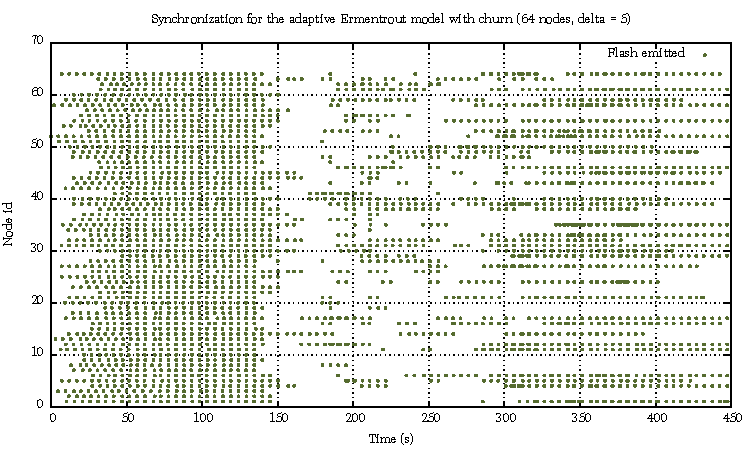
\includegraphics[scale=0.8]{../Plots/Firefly-er-64nodes-churn-d5-10.pdf}
       \caption{Adaptive Ermentrout model synchronization under churn}
       \label{fig:er-churn-sync}
     \end{figure}

     \begin{figure}[h]
       \centering
       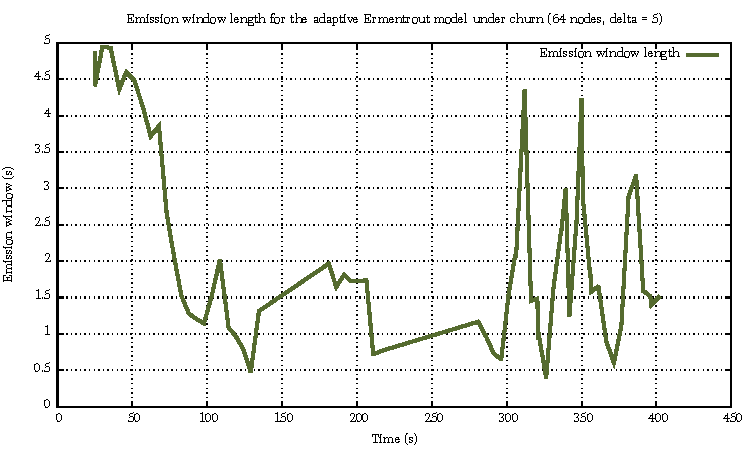
\includegraphics[scale=0.8]{../Plots/Firefly-er-64nodes-churn-d5-10-ewl.pdf}
       \caption{Adaptive Ermentrout model emission window length under churn}
       \label{fig:er-churn-ewl}
     \end{figure}

     \begin{figure}[h]
       \centering
       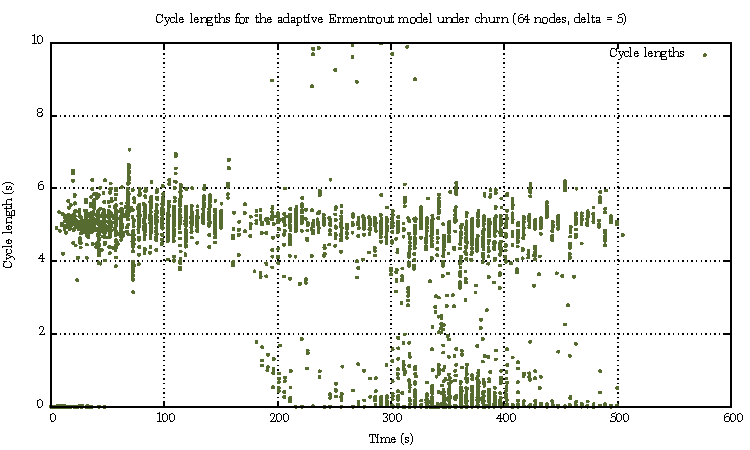
\includegraphics[scale=0.8]{../Plots/Firefly-er-64nodes-churn-d5-10-cl.pdf}
       \caption{Adaptive Ermentrout model cycle length under churn}
       \label{fig:er-churn-cl}
     \end{figure}

     

     



\section{Conclusion}
\label{sec:conclusion}

  



    
    
    












	
\end{document}



%%% Local Variables:
%%% mode: latex
%%% TeX-master: t 
%%% End:
\message{ !name(LSDS_project3_hayezl.tex) !offset(-632) }
